\def\CTeXPreproc{Created by ctex v0.2.9, don't edit!}
%\documentclass{beamer}
\documentclass[%handout,
xcolor=pdftex]{beamer}
\mode<presentation> {
  \usetheme{Warsaw}
  \setbeamercovered{transparent}
}
\let\Tiny=\tiny
\usetheme{Singapore}
\usecolortheme{dolphin}
\usepackage{amsmath}
\usepackage{textcomp}
\usepackage{amssymb}
\usepackage{amsthm}
\usepackage{graphicx}
\usepackage{color}
\usepackage{lipsum}
\usepackage{hyperref}
\usepackage{multirow}
\usepackage{bm}
%\setbeamertemplate{headline}{}
\setbeamertemplate{footline}[page number]
\newcommand\Fontvi{\fontsize{9pt}{8}\selectfont}
\newcommand\Fontvii{\fontsize{7pt}{8}\selectfont}
\newcommand{\backupbegin}{
   \newcounter{finalframe}
   \setcounter{finalframe}{\value{framenumber}}
}
\newcommand{\backupend}{
   \setcounter{framenumber}{\value{finalframe}}
}\newtheorem{proposition}{Proposition}
\title{Unit 3: Stationarity}
\author[STAT 5170: Applied Time Series, Unit 3]{Taylor R. Brown PhD}
\institute{Department of Statistics, University of Virginia}
\date{Spring 2020} %USE LEVINE LECTURE 3 FOR STRICT STATIONARITY. SHOW PROOF THAT STRICT STATIONARITY -> WEAK STATIONARITY

\AtBeginSubsection[] {
  \begin{frame}<beamer>{Outline}
    \tableofcontents[currentsection,currentsubsection]
  \end{frame}
}

\begin{document}


\frame{\titlepage}


\begin{frame}
\frametitle{Readings for Unit 3}

Textbook chapter 1.4, 1.5.

\end{frame}

\begin{frame}
\frametitle{Last Unit}
\begin{enumerate}
\item White noise.
\item Random walk model.
\item Autoregressive model.
\item Moving average model.
\item Mean function.
\item Measures of Dependence.
\end{enumerate}
\end{frame}

\begin{frame}
\frametitle{This Unit}
\begin{enumerate}
\item Stationarity
\item Autocovariance and Autocorrelation of Stationary Time Series
\item Estimating the ACF
\end{enumerate}
\end{frame}

\begin{frame}
\frametitle{Motivation}
In time series analysis, we would generally prefer to analyze a stationary sequence.  This allows us to \textbf{better estimate} autocorrelation and other quantities of interest.  One feature of stationary sequences is that they are identically distributed--but often not independent.  (Though, certainly an iid sequence is stationary.)  There are two types of stationarity: \textbf{strictly stationary} and \textbf{weakly stationary}.

\end{frame}


\section{Stationarity}
\frame{\tableofcontents[currentsection]}

\begin{frame}
\frametitle{Strictly Stationary}

A time series is \textbf{strictly stationary} if for a sequence of times $t_1, t_2,...,t_k$
$$
\{ x_{t_1},..., x_{t_k} \}
$$
has the same joint distribution as
$$
\{ x_{t_1+h},..., x_{t_k+h} \}
$$
for every integer $h$. In other words,
$$
P\{ x_{t_1}\leq c_1,..., x_{t_k} \leq c_k \}=P\{ x_{t_1+h}\leq c_1,..., x_{t_k+h}\leq c_k \}.
$$

Location does not matter--ONLY the window size.

\end{frame}


\begin{frame}
\frametitle{Weakly Stationary}

A time series $\{x_t\}$ is \textbf{ weakly stationary} if $\mu_t$ is \textbf{constant and does not depend on time $t$}, and $\gamma(s,t)$ \textbf{depends only on the distance $|s-t|$}.  \\
\vspace{5mm}
From now on when we say stationary, we'll mean weakly  stationary.  All strongly stationary time series are also weakly stationary, but the reverse may not be the case.  Most of the time we are going to be working with Gaussian time series, and in this case the two concepts coincide.
\end{frame}

\section{Autocovariance and Autocorrelation of Stationary Time Series}
\frame{\tableofcontents[currentsection]}

\begin{frame}
\frametitle{Autocovariance of Stationary Time Series}

With a stationary time series, we have the following property: $\gamma(t+h,t)=\gamma(h,0)$. So, for stationary processes we write
\begin{equation}
\gamma(h)=\mbox{E}(x_{t+h}-\mu)(x_t-\mu).
\end{equation}

We simply use the rule $\gamma(s,t)=\gamma(s-t)$. Another property of the autocovariance function when the time series is stationary is $\gamma(h)=\gamma(-h)$.

\end{frame}

\begin{frame}
\frametitle{Autocorrelation of Stationary Time Series}

For the autocorrelation function, we have
\begin{equation} \label{eq:auto}
\rho(h) =\frac{\gamma(h)}{\gamma(0)}.
\end{equation}

\end{frame}

\begin{frame}
\frametitle{White Noise}

\textbf{Question:} Show that white noise is stationary.

\vspace{50mm}

\end{frame}

\begin{frame}
\frametitle{Random Walk Process}

\textbf{Question:} Is a random walk process $\{x_t\}$ stationary? Recall from last unit I simulated three realizations of a random walk.

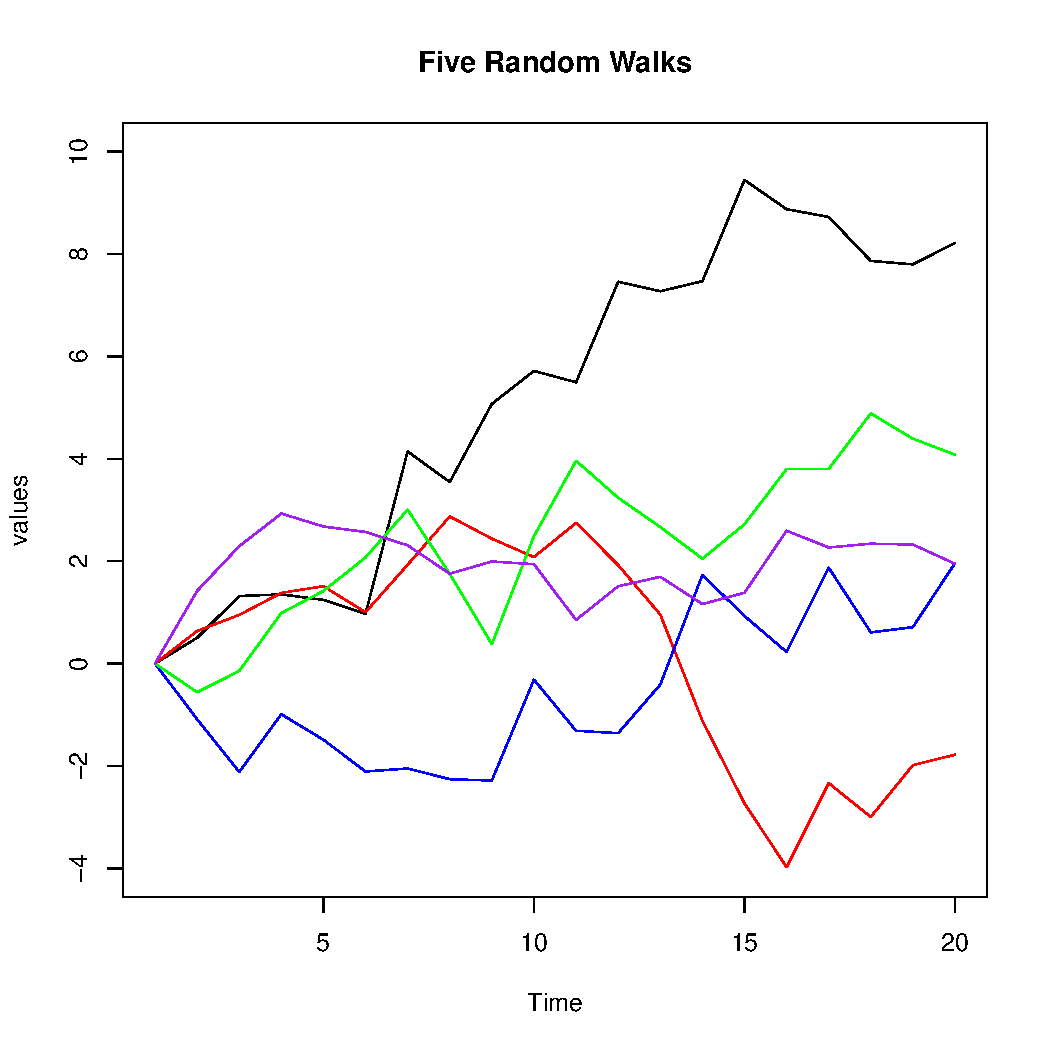
\includegraphics[width=100mm, height=60mm]{pics/randomwalk.pdf}

\end{frame}


\begin{frame}
\frametitle{MA(2) Process}

\textbf{Question:} Show that the MA(2) process is stationary.


\vspace{50mm}

\end{frame}

\begin{frame}
\frametitle{ACF of MA(2) Process}



\end{frame}

\begin{frame}
\frametitle{AR(1) Process}

\textbf{Question:} Show that if an AR(1) process is stationary, then $|\phi_1| < 1$.


\vspace{50mm}

\end{frame}

\begin{frame}
\frametitle{ACF of AR(1) Process}



\end{frame}

\section{Estimating the ACF}
\frame{\tableofcontents[currentsection]}

\begin{frame}
\frametitle{Recall Stationarity}

Suppose $\{x_t\}$ is a stationary time series. Then

\begin{itemize}
\item Its mean is \textbf{constant}.
\item Its autocovariance function is $\gamma(h)=\mbox{E}(x_{t+h}-\mu)(x_t-\mu)$. It depends only on $h=|s-t|$. This also means that the variance, $\gamma(0)$ is constant.
\item Its autocorrelation function is $\rho(h) =\frac{\gamma(h)}{\gamma(0)}$.
\end{itemize}

\end{frame}

\begin{frame}
\frametitle{Estimating the ACF}

Without stationarity, we have little
hope of estimating the full $\gamma(s,t)$.  With stationarity,
we will have \textbf{many observations} that are $h$ apart from one
another (at least when $h<<n$).  We now discuss how to
estimate $\rho(h)$ to produce ACF plots.

\end{frame}

\begin{frame}
\frametitle{Estimating the ACF}

With stationarity, the (true) mean is constant.  We can therefore estimate the mean using the \textbf{sample mean}
$$
\bar{x}=\frac{\sum_{t=1}^n x_t}{n}.
$$
This converges to $\mu$. In fact,
$$
E(\bar{x}) = E (\frac{\sum^n_{t=1}x_t}{n}) = \frac{1}{n} \sum^n_{t=1} E(x_t)  =\frac{1}{n} \sum^n_{t=1} \mu =\mu.
$$
\end{frame}

\begin{frame}
\frametitle{Estimating the ACF}

Consider the \textbf{sample autocovariance function}
\begin{equation} \label{eq:samp1}
\hat{\gamma}(h)=\frac{\sum_{t=1}^{n-h} (x_{t+h}-\bar{x})(x_{t}-\bar{x})}{n}.
\end{equation}
for $h=0,1,...,n-1$.  \\
\vspace{5mm}
For fixed $h$, all the random variables $y_t=(x_{t+h}-\bar{x})(x_{t}-\bar{x})$ have the same distribution (\textbf{due to stationarity}).  Therefore, $\frac{\sum_{t=1}^{n-h} y_t}{n}$ converges to $\gamma(h)=E(x_{h}-\mu)(x_{0}-\mu)$.

\end{frame}

\begin{frame}
\frametitle{Estimating the ACF}

To obtain the \textbf{sample autocorrelation} we simply scale by the variance
\begin{equation} \label{eq:samp2}
\hat{\rho}(h)=\frac{\hat{\gamma}(h)}{{\hat{\gamma}(0)}}.
\end{equation}

One thing to notice in the sample autocovariance function (\ref{eq:samp1}) is that we divide by $n$ not $n-h$ or $n-1$.  This ensures that if we calculate variances, they are all positive.

\end{frame}


\begin{frame}
\frametitle{Sample ACF}

We can recognize the sample ACF of time series.\\

\begin{center}
\begin{tabular}{ r l }
  \textbf{Time series} & \textbf{ACF} \\
White noise & 0\\
Trend & Slow decay\\
Periodic & Periodic\\
MA(q) & 0 for $h>q$\\
AR(p) & Decays to 0 exponentially\\
\end{tabular}
\end{center}

\end{frame}

\begin{frame}
\frametitle{Sample ACF for Gaussian White Noise}

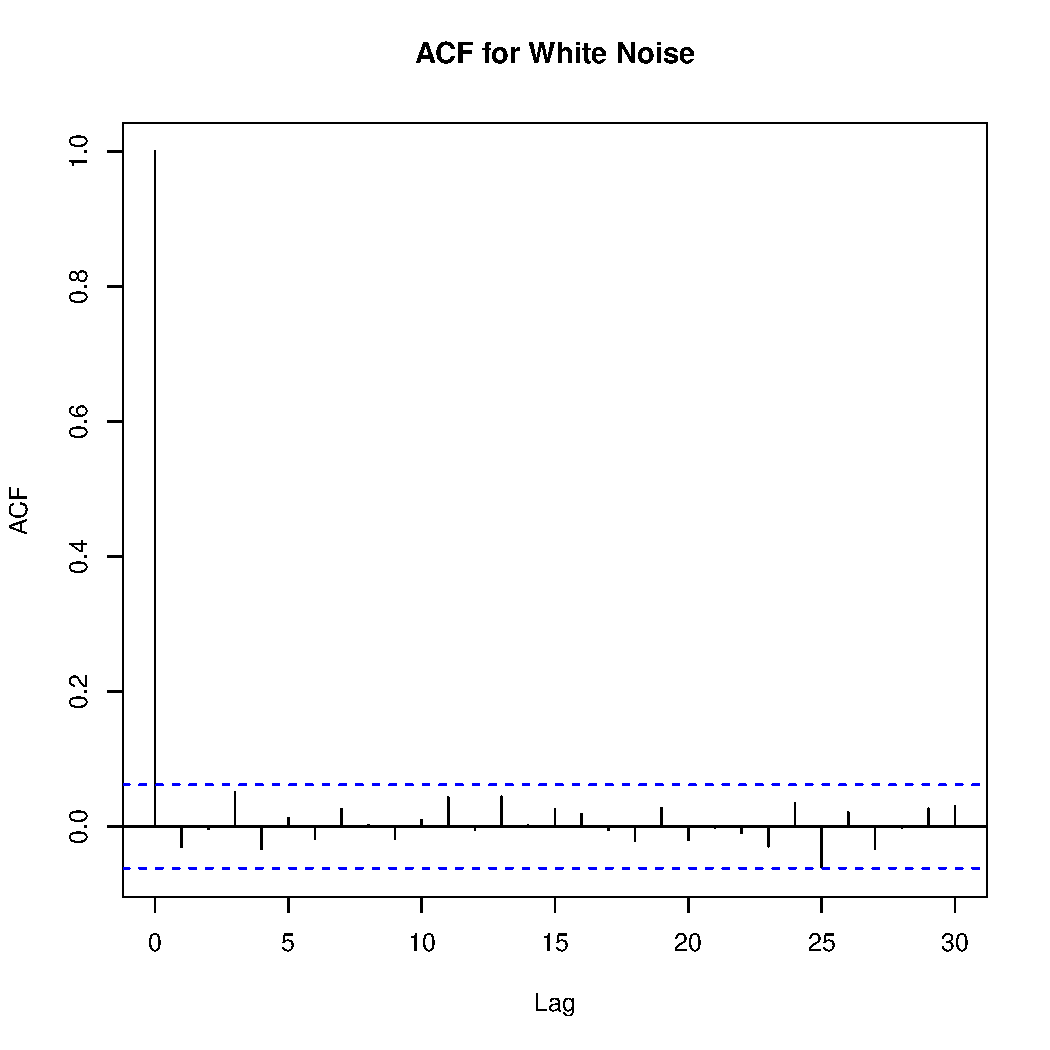
\includegraphics[width=100mm, height=80mm]{pics/acf_wn.pdf}

\end{frame}

\begin{frame}
\frametitle{Sample ACF for Gaussian White Noise}

When the true model is white noise $\hat{\rho}(h)$ is approximately normally distributed with zero mean and standard deviation of $1/\sqrt{n}$.

\end{frame}


\begin{frame}
\frametitle{Sample ACF: Marriages in Church of England}

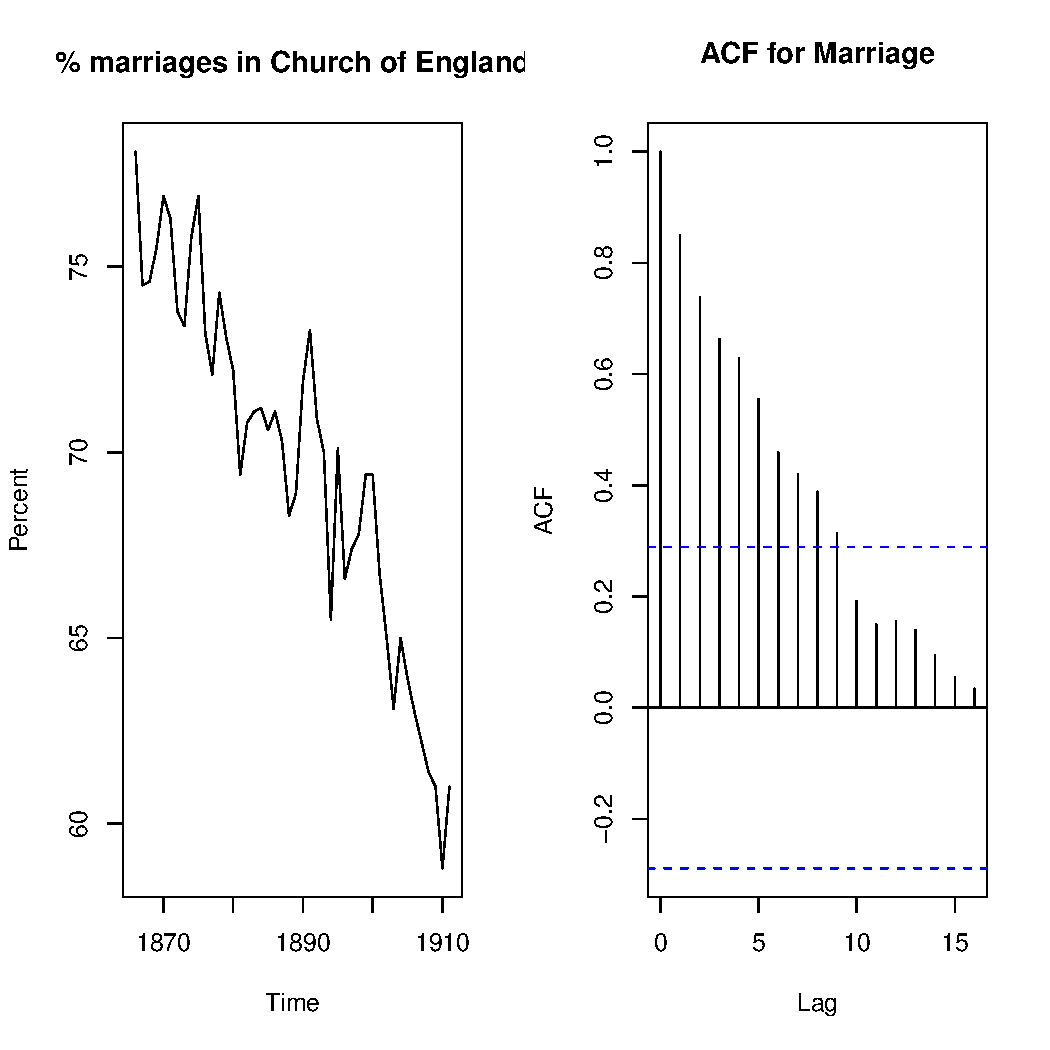
\includegraphics[width=100mm, height=80mm]{pics/acf_marriage.pdf}

\end{frame}

\begin{frame}
\frametitle{Sample ACF: Average Monthly Temperature in Dubuque, IA}

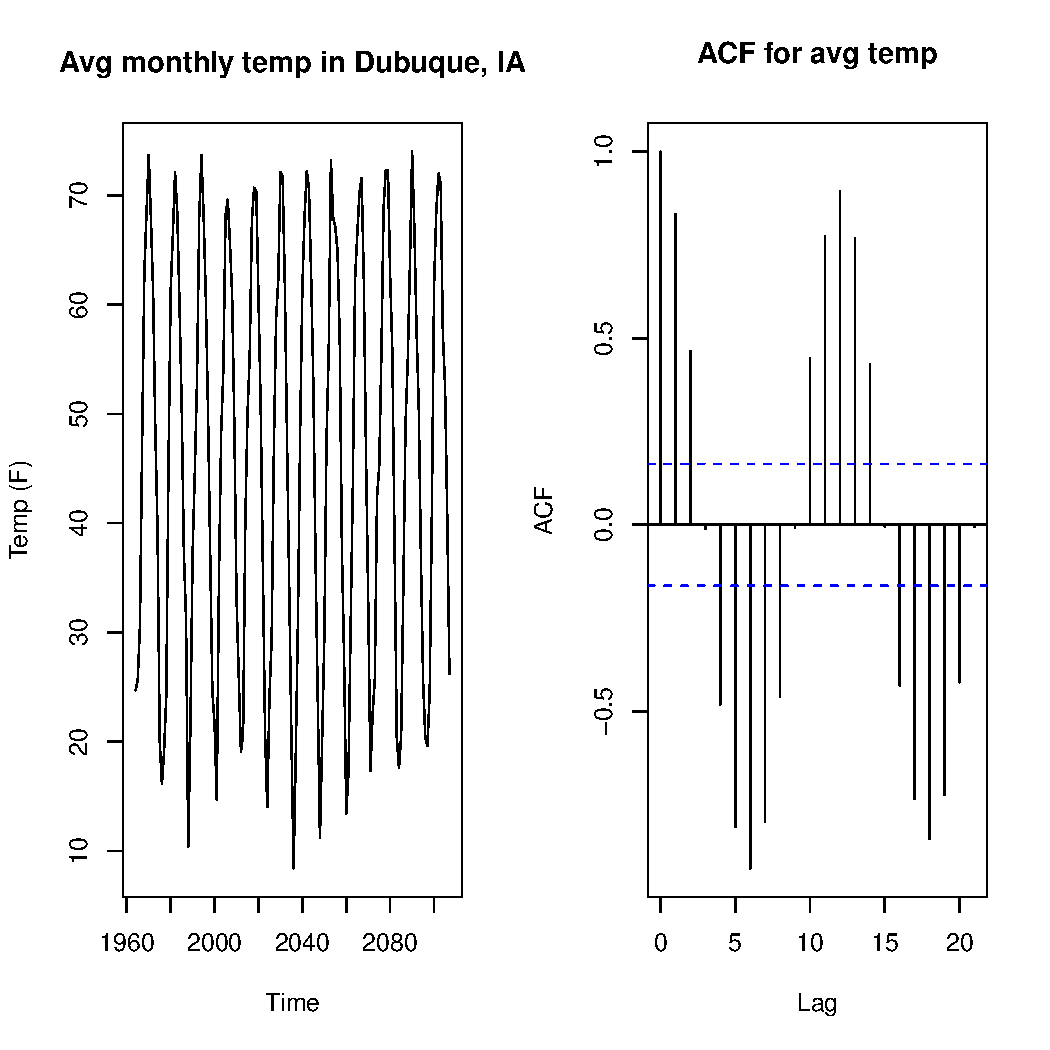
\includegraphics[width=100mm, height=80mm]{pics/acf_dubuque.pdf}

\end{frame}

\begin{frame}
\frametitle{Sample ACF: MA(1) Process}

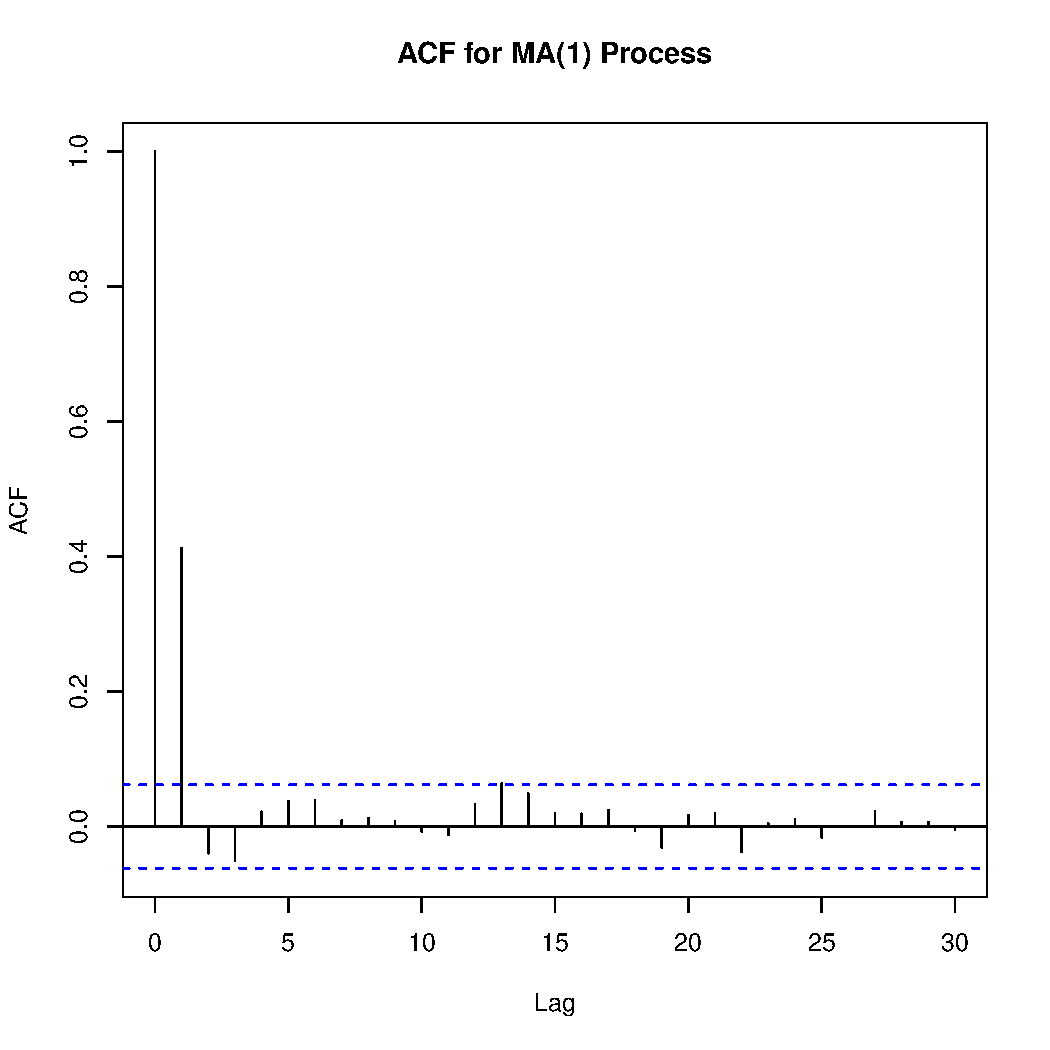
\includegraphics[width=100mm, height=80mm]{pics/acf_ma1.pdf}

\end{frame}

\begin{frame}
\frametitle{Sample ACF: AR(1) Process}

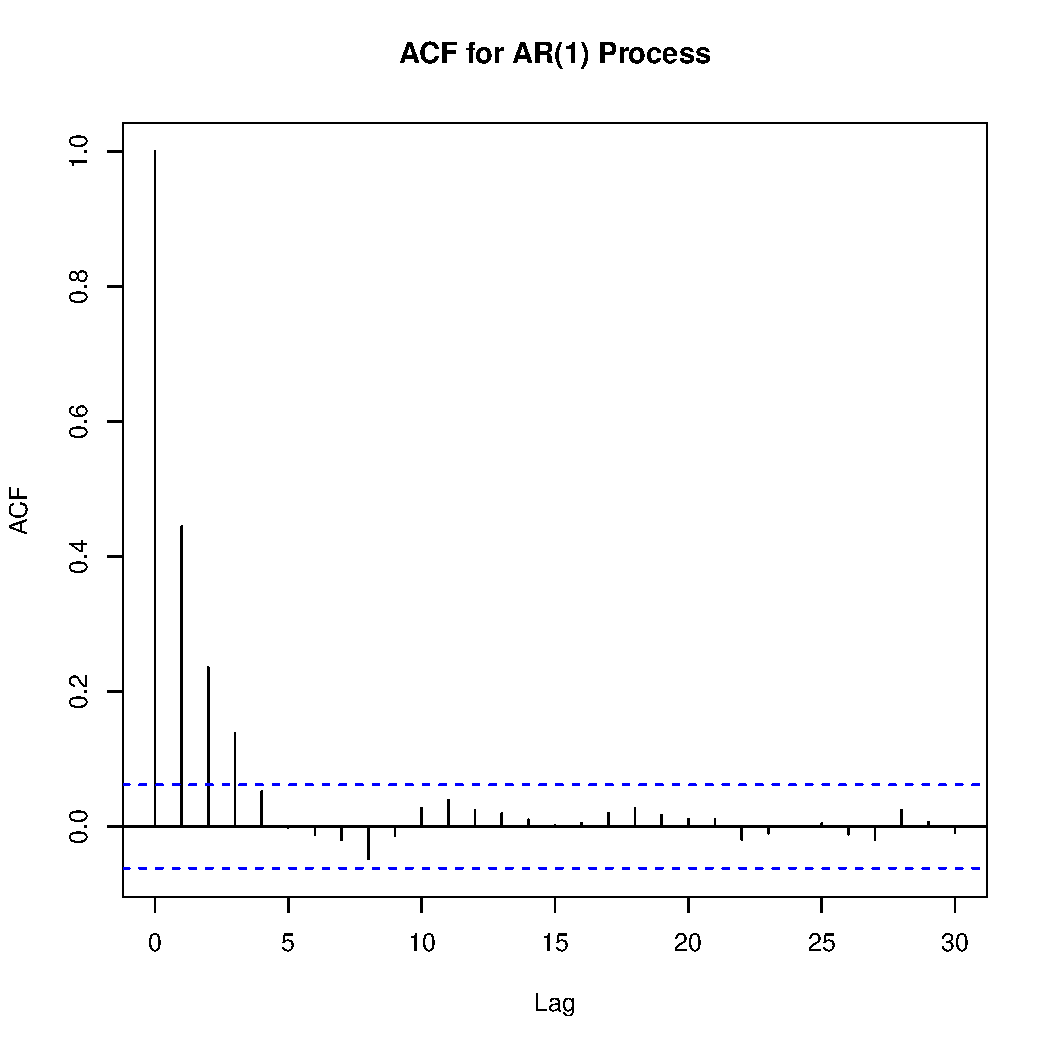
\includegraphics[width=100mm, height=80mm]{pics/acf_ar1.pdf}

\end{frame}



\end{document} 